\documentclass[10pt,a4paper]{amsart}
\usepackage[margin=19mm]{geometry}
\usepackage{amsmath,amssymb,mathtools}
\usepackage[scr=rsfs,cal=euler]{mathalfa}
\usepackage{xfrac}
\usepackage[unicode,hidelinks,bookmarks=false]{hyperref}
\newcommand{\ie}{i.e.\ }
\newcommand{\cf}{cf.\ }
\newcommand{\resp}{respectively\ }
\newcommand{\Subsection}{\subsection}
\providecommand{\nobreakdash}{\nobreak\hbox{-}}
\setlength{\emergencystretch}{2em}
\multlinegap0pt
\usepackage{tikz}
\usepackage{amssymb}
\usepackage[shortlabels]{enumitem}
\newtheorem{defn}{Definition}
\newtheorem{lemma}{Lemma}
\newtheorem{corollary}{Corollary}
\newtheorem{theorem}{Theorem}
\newcommand{\D}{\Delta}
\newcommand{\RP}{\mathbb{RP}}
\newcommand{\Sp}{\mathbb{S}}
\def \ZZ{{\bb{Z}}}
\def \bb{\mathbb}
\title{On the equivariant triangulation of some small covers}
\author{Raju Kumar Gupta, Soumen Sarkar}
\date{Source: arXiv:2602.12857v1 (CC BY 4.0)}
\begin{document}
\maketitle

\noindent\emph{Source and licence.} On the equivariant triangulation of some small covers. Version arXiv:2602.12857v1 (CC BY 4.0), distributed by arXiv under the Creative Commons Attribution 4.0 International licence, http://creativecommons.org/licenses/by/4.0/, as recorded in the arXiv licence metadata for this exact version and shown on the abstract page https://arxiv.org/abs/2602.12857v1. Full licence notice: \texttt{licenses/arxiv-2602.12857-CC-BY-4.0.txt}.\par\smallskip

\noindent\textit{Editorial scope.} Counted unit: the article's theorem thm7 (source0.tex lines 1097--1099). The article's complete original proof of it is delivered with it (source0.tex lines 1100--1304, one \texttt{proof} environment of 205 lines). No mathematics is written, repaired or re-derived: the statement and the proof are the article's own lines, in the article's own notation, and no retained line is substituted or re-flowed.  Retained uncounted as the source-local context the proof needs: lines 282--296; lines 319--321; lines 452--462; lines 552--556; lines 616--618; lines 626--631; lines 1042--1044; lines 1068--1070.  Nothing was omitted from any retained span, so the package carries no omission record.  No retained line contains a citation, so the wrapper carries no bibliography and no bibliography entry.  The retained lines contain the article's own diagram code, which the wrapper typesets with the standard tikz packages; no image file is delivered and the package declares no asset dependency.  Editorial formatting only, in addition: an AMS \texttt{amsart} preamble that restates the article's own declarations and macros used by the retained lines, namely the environments \texttt{defn}, \texttt{lemma}, \texttt{corollary}, \texttt{theorem} on separate counters, together with the standard packages those lines need.  The retained environments print in this document as Definition 1, Lemma 1, Corollary 1, Theorem 1 in order of appearance, whereas the article prints the same items with the numbering of its own full document.  The complete native source of the article as distributed in the arXiv e-print for this exact version is bundled unchanged as \texttt{sources/194587/source0.tex}.
\begin{defn}\label{Charecteristic}
Let $\{\mu_1, \ldots, \mu_n\}$ be the standard generators of $\ZZ_2^n$.
Let $$X_i := \{[x_1: \cdots : x_n] \in \mathbb{RP}^n : x_i=0 ~\mbox{in}~ Q_n\}~ \mbox{for}~ i= 1, \ldots, n,$$
and $$X_0 := \{[x_1 : \cdots : x_n] \in \mathbb{RP}^n : (x_1, \ldots, x_n) \in \partial Q_n\}.$$ 
Then $X_0, X_1, \ldots, X_{n-1}$ and $ X_n$ are codimension one submanifold of $\mathbb{RP}^n$ fixed by the subgroups
$(\mu_1+ \cdots + \mu_n), (\mu_1), \ldots, (\mu_{n-1})$ and $(\mu_n)$, respectively. 

Let $\pi \colon \mathbb{RP}^n \to \Delta^n$ be the orbit map of the standard $\ZZ_2^n$-action on $\mathbb{RP}^n$. 
Let $F_i$ be the $(n-1)$-dimensional face in $\Delta^n$ not containing the vertex $e_i$ for $i=0, \ldots, n$. Then, $F_i := \pi(X_i)~\mbox{for}~ i= 0, \ldots, n$.
Thus, there is an assignment 
$$F_0 \to \mu_1+ \cdots + \mu_n:=\xi_0 ~\mbox{and} ~ F_i \to \mu_i :=\xi_i ~ \mbox{for}~ i =1, \ldots, n.$$
This assignment is called a $\ZZ_2$-{\em characteristic function} on $\Delta^n$ and $\xi_i$
is called a $\ZZ_2$-characteristic vector corresponding to the face $F_i$. 

\end{defn}

\begin{lemma}\label{lem3}
Let $X$ be a $\ZZ^{n}_2$-equivariant triangulation of $\Sp^{n-1}$ for some $n\geq 2$. Then $\mathrm{Card}(V(X))$ is even and $\mathrm{Card}( V(X)) \geq 2n$
\end{lemma}

\begin{corollary}\label{8vertex}
Let $X$ be a $\mathbb{Z}_2^4$-equivariant triangulation of $\mathbb{S}^3$ with $8$ vertices. 
Then the only possibility for the vertex set $V(X)$ is (up to permutation of coordinates) one of the following for some fixed $a,b,c,d \in\mathbb{R}\setminus\{0\}$.
$$
\begin{aligned}
&(I)\quad  V(X) = \{(\pm a,\pm b,0,0),\ (0,0,\pm c,\pm d)\} \subset \mathbb{S}^3.\\
&(II)\quad V(X) = \{(\pm a,\pm b,0,0),\ (0,0,\pm 1,0),\ (0,0,0,\pm 1)\} \subset \mathbb{S}^3.\\
&(III)\quad V(X) = \{(\pm 1,0,0,0),\ (0,\pm 1,0,0),\ (0,0,\pm 1,0),\ (0,0,0,\pm 1)\}.
\end{aligned}
$$
\end{corollary}

\begin{theorem}\label{thm2}
Let $M$ be an $n$-dimensional small cover.
Let $X$ be a $\ZZ_2^n$-equivariant triangulation of $M$ and $\pi \colon |X|\rightarrow P$ is the orbit map where $P$ is a simple polytope. Then the collection
$\{\pi(\sigma) \colon \sigma \in X ~ \mbox{and}~ \dim{\sigma} = n\}$ gives a triangulation of the polytope $P$.
\end{theorem}

\begin{lemma}\label{lem1}
Let $X$ be a $\ZZ_2^n$-equivariant triangulation of $\mathbb{RP}^{n}$. If $e_0, \ldots, e_{n}$ are fixed points of $|X|$, then $\mathrm{Card}(V(X)\setminus \{e_i : i=0, \ldots, n\})$ is even. 
\end{lemma}

\begin{lemma}\label{lem4}
Let the notations be same as in Definition 
\ref{Charecteristic}. Let $X$ be a $\ZZ_2^n$-equivariant triangulation of $\mathbb{RP}^n$ and $\sigma$ be an $n$-simplex
in $X$ such that $e_i \in |\sigma|$ for some $i \in \{0, \ldots, n\}$. Then $V(\sigma) \cap
X_i$ is empty.
\end{lemma}

\begin{lemma}\label{lem:nointerior}
   Let $X$ be a $\ZZ_2^4$-equivariant triangulation of $\RP^4$ with less than 18 vertices. Let $\pi:|X|\rightarrow \D^4$ be the orbit map. There is no face of dimension three or more in $\D^4$ whose interior conatins a point $x$ such that $\pi^{-1}(x) \cap V(X) \neq \emptyset$. 
\end{lemma}

\begin{lemma}\label{atmost9}
Let $X$ be a $\ZZ_2^4$-equivariant triangulation of $\RP^4$.  If $f_0(X)\leq 17$ then for any $3$-simplex $\sigma$ in $\D^4$, $\pi^{-1}(\sigma)$ contains at most $9$ vertices. Moreover, for $x\in V(\D^4)\setminus V(\sigma)$, $Card(V(\partial D_x))=8$. 
\end{lemma}

\begin{theorem}\label{thm7}
 There is no $\ZZ_2^4$-equivariant triangulation of $\mathbb{RP}^4$ with at most $17$ vertices.
\end{theorem}

\begin{proof}
Let $X$ be a $\ZZ_2^4$-equivariant triangulation of $\mathbb{RP}^4$ with $16$ vertices.  By Lemma \ref{lem1}, number of vertices in $R =V(X)\setminus \{e_0,\ldots,e_4\}$ is even. First, assume that $V(X)$ does not contain any fixed vertex. For each $i\in \{0,\ldots,4\}$, $V(\partial D_i)\subseteq V(X)$ and  by Lemma \ref{lem3}, $\mathrm{Card}( V(\partial D_i)) \geq 8$. Further, $e_i\notin \partial D_i$ for all $i\in \{0,\ldots,4\}$. This implies that $\bigcup_{i=0}^{4}(V(\partial D_i))=R$.


$\textbf{Case 1}:$ Suppose that $\mathrm{Card}(V(\partial  D_i)) \geq 14$  for some $i \in \{0, \ldots, 4\}$.

If $\mathrm{Card}(V(\partial D_j)) = 8$ for some $j\neq i$, then by Corollary~\ref{8vertex}, $\pi(V(\partial D_j))$ lies in one of the following configurations:  
\begin{itemize}
    \item[(i)] Interiors of four edges of $\D^4$ containing the vertex $v_j$.

    \item [(ii)]  Interiors of two edges containing $v_j$ and one complementary triangle containing $v_j$ in $\Delta^4$.

    \item  [(iii)] Interior of two complementary triangles containing $v_j$ in $\Delta^4$.
\end{itemize}
   
   However, since $\mathrm{Card}(V(\partial D_j) \cap V(\partial D_i)) \ge 6$, at least $6$ vertices of $V(\partial D_j)$ must come from the interiors of some faces in $\D^4$ containing $v_iv_j$. From the above configurations, this is not possible.
Hence, we conclude that $\mathrm{Card}(V(\partial D_j)) \ge 10$.

Now, since $\mathrm{Card}(V(\partial D_j) \cap V(\partial D_i)) \ge 8$ for all $j \neq i$, the pigeonhole principle implies that  
$V(\partial D_i) \cap V(\partial D_k) \cap V(\partial D_l) \cap V(\partial D_m) \neq \emptyset$  
for some distinct $i, k, l, m \in \{0,1,2,3,4\}$. This means that there exists a point $z$ in the interior of a simplex in $\D^4$ containing the vertices $e_i, e_k, e_l, e_m$ such that $\pi^{-1}(z) \subseteq V(\partial D_i)$. This contradicts Lemma~\ref{lem:nointerior}. Hence, there is no $i \in \{0,1,2,3,4\}$ such that $\mathrm{Card}(V(\partial D_i)) \ge 14$.



$\textbf{Case 2}:$ Suppose that $\mathrm{Card}(V(\partial D_i))= 12$ for some $i\in \{0,1,\ldots,4\}$. 

The points of $\pi(V(\partial D_i))$ lie either in the interiors of triangles or in the interiors of edges, by Lemma~\ref{lem:nointerior}, . For each point $x\in \pi(V(\partial D_i))$ in the interior of the triangle, $\pi^{-1}(x)$ consists of four vertices in $\partial D_i$, and for each point $x\in \pi(V(\partial D_i))$ in the interior of an edge, $\pi^{-1}(x)$ consists of two vertices in $\partial D_i$.

If there exists a vertex that belongs to four or more of the sets $V(\partial D_j)$ for $j\in\{0,\ldots,4\}$, then there exists an interior point $x$ in a $3$-simplex $\sigma$ such that $\pi^{-1}(x)$ contains a vertex of $X$. This contradicts Lemma~\ref{lem:nointerior}. Hence, each vertex of $X$, except for the fixed vertex, lies in at most three of the sets $V(\partial D_j)$ for $j\in\{0,\ldots,4\}$.

Thus, the total multiplicity of the vertices is at most $16 \times 3 = 48$. Therefore, $\sum_{j \in \{0,1,2,3,4\}} \mathrm{Card}(V(\partial D_j)) \le 48$. This implies that $\sum_{j \ne i} \mathrm{Card}(V(\partial D_j)) \le 36$. 

Let $j, k, l, m$ denote the remaining four elements of $\{0,1,2,3,4\} \setminus \{i\}$. Since $\mathrm{Card}(V(\partial D_s)) \ge 8$ and is even for each $s \ne i$, the possible tuples $(\mathrm{Card}(V(\partial D_j)), \mathrm{Card}(V(\partial D_k)), \mathrm{Card}(V(\partial D_l)), \mathrm{Card}(V(\partial D_m)))$ are $(8,8,8,8)$, $(8,8,8,10)$, $(8,8,8,12)$, or $(8,8,10,10)$.

Observe that for the first three possibilities, there exists some $s \in \{j, k, l\}$ such that either $V(\partial D_s)$ intersects $V(\partial D_i)$ in more than four vertices, or there exists a common vertex in $V(\partial D_s)$ for $s \in \{j, k, l, m\}$, contradicting Corollary~\ref{8vertex} or Lemma~\ref{lem:nointerior}, respectively. Hence, we are left with the only possible case $(8,8,10,10)$.

It follows that $V(\partial D_j)$ and $V(\partial D_k)$ intersect $V(\partial D_i)$ in exactly four vertices each, and $V(\partial D_j)$ and $V(\partial D_k)$ intersect each other in exactly four vertices from $V(X) \setminus V(\partial D_i)$. This implies that the interior of the triangle $e_j e_k e_s$ in $\D^4$ contributes four vertices to both $V(\partial D_j)$ and $V(\partial D_k)$ for some $s \in \{l, m\}$. 

By Corollary~\ref{8vertex}, for some $t \in \{l, m\} \setminus \{s\}$, the interiors of triangles $e_j e_i e_t$ and $e_k e_i e_t$ contribute four vertices to $V(\partial D_j)$ and $V(\partial D_k)$, respectively. Since $V(\partial D_t)$ contains $10$ vertices, there is a $p\neq t$ such that the interior of $e_pe_t$ contribute at least two vertices to the $V(\partial D_t)$. If $p=i,p=j$, or $p=k$, then the $3$-simplex $e_je_ke_ie_t$ contribute at least $10$ vertices to the $V(X)$. This contradicts Lemma \ref{atmost9}. Thus, the interior of $e_te_s$ must contribute at least two vertices to the $V(\partial D_t)$. Since from Lemma \ref{lem4}, $V(\pi^{-1}(e_je_ke_se_t))\cap V(\partial D_i)=\emptyset $, and $\bigcup_{r=0}^{4}\partial D_r$ contains at most $16$ vertices, $\mathrm{Card}(V(\partial D_i))\leq 10$. This is a contradiction.



$\textbf{Case 3}:$ Suppose that $\mathrm{Card}(V(\partial D_i)) = 10$ for some $i\in \{0,1,\ldots,4\}$. 

If $\mathrm{Card}(V(\partial D_j)) = 10$ for all $j \in \{0,1,2,3,4\}$, then some vertex must belong to at least four of the sets $V(\partial D_j)$, contradicting Lemma~\ref{lem:nointerior}. Hence, there exists $s \ne i$ such that $\mathrm{Card}(V(\partial D_s)) = 8$. Since $\mathrm{Card}(V(\partial D_j)) = 10$, the vertex distribution for $\partial D_j$ is one of the following:
\begin{itemize}
    \item [(i)] Eight vertices comes from the interiors of triangles containing $e_j$ in $\D^4$ and two vertices comes from the interior of an edge containing $e_j$ in $\D^4$.

    \item [(ii)] Four vertices comes from the interior of a triangle containing $e_j$ and the remaining $6$ vertices comes from the interiors of  edges containing $e_j$ in $\D^4$.
\end{itemize}

\textbf{Subcase (i):} Suppose that the  eight vertices of $V(\partial D_i)$ comes from the interiors of triangles in $\D^4$.  


Suppose that both the triangles belong to a tetrahedron $\sigma$ with $V(\sigma) = \{e_i, e_j, e_k, e_l\}$.  
If both triangles contributing to $V(\partial D_i)$ are the same, say $e_i e_j e_k$, then the  tetrahedron $e_i e_j e_k e_m$ for some $m \notin \{i,j,k,l\}$ would contribute more than nine vertices to $V(X)$, contradicting Lemma~\ref{atmost9}.  
Hence, two distinct triangles of $\sigma$, say $e_i e_j e_k$ and $e_i e_j e_l$, each contribute four vertices to $V(\partial D_i)$.

The remaining two vertices of $V(\partial D_i)$ must then come from the interior of an edge $e_i e_m$, where $m \notin  \{i,j,k,l\}$.  Since $V(\pi^{-1}(e_ie_je_ke_l))\cap V(\partial D_m)=\emptyset$, by Lemma~\ref{lem3}, $\mathrm{Card}(V(\partial D_m)) = 8$, and the interior of the edge $e_i e_m$ also contributes two vertices to $V(\partial D_m)$.  Thus, $\partial D_m$ must be either of type Corollary \ref{8vertex} $(II)$ or $(III)$. 
If $\partial D_m$ is of type  Corollary~\ref{8vertex} $(III)$, then the interiors of $e_m e_j$, $e_m e_k$, and $e_m e_l$ each contribute two vertices to $V(\partial D_m)$, so the tetrahedron $e_i e_j e_k e_m$ would contribute at least ten vertices to the $V(X)$, a contradiction. Now, suppose that $\partial D_m$ is of type   Corollary \ref{8vertex} $(II)$. Then the following situation arises.
\begin{itemize}
\item Let interior of the edge $e_je_m$ and interior of triangle $e_ke_le_m$ contribute two and four vertices to the $\partial D_m$, respectively. Since $R$ contains at most $16$ vertices and the interiors of faces $e_ie_je_k,e_ie_je_l,e_ke_le_m,e_ie_m,e_je_m$ contribute the $16$ vertices to $X$, $\partial D_k$ as well as $\partial D_l$ contain $8$ vertices and are of type Corollary \ref{8vertex} $(I)$. On the other hand, if $\partial D_j$ contains $8$ vertices then its vertices arise from the interior of faces $e_ie_je_k$ and $e_ie_je_l$  which are not complementary faces containing $e_j$. Thus, $\partial D_j$ contains  $10$ vertices. Now, since the vertices of $\partial D_k$ arise form the interior of $e_ie_je_k$ and $e_ke_le_m$, without loss of generality assume that the vertex set of $\partial D_k$ is $\{(\pm a,\pm b,0,0),(0,0,\pm c,\pm d)$, for some non-zero real numbers $a,b,c,d$. Now, since the same interior point of $e_ke_le_m$ contributes vertices to the $\partial D_l$, $\{(0,0,\pm c,\pm d)\}\subset  V(\partial D_l)$. Thus, the other four vertices of $\partial D_l$ must be of type $\{(\pm e, \pm f,0,0)\}$ for some non-zero $e,f$ and corresponding to the face $e_ie_je_l$. Since the vertices of $\partial D_i$ arise from the interios of faces $e_ie_je_k,e_ie_je_l$, and $e_ie_m$, $\{(\pm a,\pm b,0,0),(\pm e, \pm f,0,0) \}\subset V(\partial D_i)$. The other two vertices of $\partial D_i$ comes from the interior of the edge $e_ie_m$, thus these two vertices must be antipodal and contains exactly one non-zero cordinate. Therefore for any choices of the two vertices arising from $e_ie_m$, all vertices of $V(\partial D _i)$ contains a zero coordinate, which is not possible. 

\item If interior of the edge $e_ke_m$ (resp., $e_le_m$) and interior of triangle $e_je_le_m$ (resp., $e_je_ke_m$) contribute two and four vertices to the $\partial D_m$, respectively, then the $3$-simplex $e_ie_je_le_m$ (resp., $e_ie_je_ke_m)$ contribute at least $10$ vertices to the $V(X)$. This situation is not possible.

 
\end{itemize}

Now, consider that the two triangles whose interiors contribute $8$ vertices to the $\partial D_i$ are from two different tetrahedrons. Then both triangles must be complementary triangles containing $e_i$. Let the interiors of $e_ie_je_k$ and $e_ie_le_m$ contribute $8$ vertices to the $\partial D_i$. Without loss of generality, assume that the other two vertices of $\partial D_i$ comes from the interior of the edge $e_ie_j$. 
Since the $2$-simplex $e_ie_je_k$ contribute at least $6$ vertices to the $V(X)$, the  interior of $e_ie_le_m$ must contribute four vertices to the $\partial D_l$ and $\partial D_m$ both. If $\partial D_m$ is of type Corollary \ref{8vertex} $(II)$, then the interiors of $e_je_m$, $e_ke_m$ contribute the other four vertices to the $\partial D_m$. Then the $3$-simplex $e_ie_je_ke_m$ contributes at least $10$ vertices to the $V(X)$, which is a contradiction. Now, assume that $\partial D_m$ is of type Corollary \ref{8vertex} $(I)$. Then the other four vertices arise from the interior of $e_je_ke_m$. Then again the $3$-simplex $e_ie_je_ke_m$ contributes at least $10$ vertices to the $X$. This is a contradiction. Hence, this subcase is not possible.

\textbf{Subcase (ii):} Suppose that only one triangle, say $e_i e_j e_k$, contributes four vertices to $V(\partial D_i)$.  
Let $e_l, e_m$ be the remaining vertices of $\mathbb{D}^4$.  
If the remaining six vertices of $V(\partial D_i)$ come from edges or triangles within $e_i e_j e_k e_l$ or $e_i e_j e_k e_m$, then by Lemma~\ref{atmost9}, $V(X)$ would have more than nine vertices, a contradiction.  
Thus, at most two of these vertices can come from edges of $e_ie_je_k$ containing $e_i$.

Assume $e_i e_j$ contributes two such vertices.  
Then by Lemma~\ref{lem3}, edges $e_ie_l$ and $e_ie_m$ also contribute two vertices each to $V(\partial D_i)$. Now, since the $3$-simplex $e_ie_je_ke_l$ contributes at least $8$ vertices to the $X$, $\mathrm{Card}(V(\partial D_m)) = 8$ and the interior of $e_ie_m$ must contribute $2$ vertices to the $\partial D_m$.   
If $\partial D_m$ is of type Corollary \ref{8vertex} $(III)$ , then the interiors of $e_m e_j$, $e_m e_k$, and $e_m e_l$ each contribute two vertices to $V(\partial D_m)$, forcing $e_i e_j e_k e_m$ to contribute at least  ten vertices to $X$, again a contradiction.  
Suppose that $\partial D_m$ is of type Corollary \ref{8vertex} $(II)$. Then for any vertex distribution of $\partial D_m$ in $\D^4$, $e_ie_je_ke_m$ contribute at least $10$ vertices to the $X$, a contradiction.




Finally, if no edge of $e_i e_j e_k$ containing $e_i$ contributes vertices to $V(\partial D_i)$, then the remaining six vertices must come from the interiors of $e_i e_l$ and $e_i e_m$, which 
If the interior of $e_ie_l$ or $e_ie_m$ contribute $6$ verices then either $e_ie_je_ke_l$ or $e_ie_je_ke_m$ contribute at least $10$ vertices to $X$, a contradiction. Thus, we assume that four vertices comes from the interior of $e_ie_l$ and two vertices comes from the $e_ie_m$. Then since the $3$-simplex $e_ie_je_ke_l$ contribute at least  $8$ vertices to the $X$, $\partial D_m$ is of type Corollary \ref{8vertex}$(II)$or $(III)$ . If it is of type Corollary \ref{8vertex} $(III)$ , then $e_ie_je_ke_m$ contribute $10$ vertices to the $X$, a contradiction. Suppose that $\partial D_m$ is of type Corollary \ref{8vertex} $(II)$. Then for any distribution of vertices of $\partial D_m$, either $e_i{e_j}e_{k}e_{m}$, $e_{i}e_{j}e_{l}e_{m}$ or $e_{i}e_{k}e_{l}e_{m}$ contribute at least $10$ vertices to the $X$, a contradiction.

Hence, all possible configurations lead to contradictions.





$\textbf{Case 4}:$ Suppose that $\mathrm{Card}( V(\partial D_i)) = 8$  for $i=0, \ldots, 4$. 

Fix an $i \in \{0, \ldots, 4\}$. Then, there are $3$ possibilities for the triangulation of $\partial D_i$ as described in Corollary \ref{8vertex}. 
If the vertex set of $\partial D_i$ is of type Corollary \ref{8vertex} $(III)$ for some $i\in \{0,1,2,3,4\}$, then $\pi(V(\partial D_i))$ belongs to the interiors of edges of $\Delta^4$ containing the vertex $e_i$, and thus interior of each edge contribute two vertices to the $V(\partial D_i)$. Now, if the vertex set of $\partial D_x$ is of type Corollary \ref{8vertex} $III$ for all $x\in \{0,1,2,3,4\}\setminus \{i\}$
 then interior set  of each edge of $\D^4$ contributes two vertices to the $V(X)$ and then $X$ has at least $20$ vertices. This is a contradiction.
Let for some $j\neq i$, $e_je_le_m$  contributes four vertices to the $\partial D_j$. If $i\in \{l,m\}$ then $e_ie_je_pe_q$ contribute at least $10$ vertices to the $V(X)$ for some $p\in \{l,m\}\setminus \{i\}$ and $q\in \{0,1,2,3,4\}\setminus \{i,j,p\}$. This is a contradiction. If $i\notin\{l,m\}$, then the simplex $e_ie_je_le_m$ contribute at least $10$ vertices to the $V(X)$. This is a contradiction. This implies that for any $x\in \{0,1,2,3,4\}\setminus \{i\}$, $\partial D_x$ cannot be of type Corollary \ref{8vertex} $(I)$ or $(II)$.

Suppose that the vertex set of $\partial D_x$ for all $x\in\{0,\ldots,4\}$ is of type Corollary \ref{8vertex} $(I)$. Let for some $i\in\{0,1,2,3,4\}$, interiors of the  $2$-simplices, say $e_ie_je_k$ and $e_ie_le_m$ in $\D^4$   contributes $8$ vertices to the $V(\partial D_i)$ where $j,k,l,m$ are distinct numbers from $\{0,1,2,3,4\}\setminus \{i\}$. Now, we have the following situations.

\begin{itemize}
    \item The interior of $e_ie_je_k$  does not contribute the same four vertices of $\partial D_i$ to $\partial D_j$. Thus, interior of $e_je_le_m$   also does not contribute any vertex to $V(\partial D_j)$. Let the interiors of $e_je_ke_l$ and $e_je_ie_m$ contribute the $8$ vertices to $\partial D_j$. Then the $16$ vertices of $V(X)$ comes from the interior of faces $e_ie_je_k$, $e_ie_le_m$, $e_je_ke_l$ and $e_ie_je_m$. Then from Corollary \ref{8vertex}, we find that the interiors of $e_ie_le_m$,  and $e_ie_je_m$ cannot contribute the $8$ vertices to the $\partial D_m$ as they are not complementary triangles containing $e_m$. Thus, this case is not possible. Similarly, this case is not possible if the interiors of $e_je_ie_l$ and $e_je_ke_m$ contribute the $8$ vertices to $\partial D_j$.
    
   \item The interior of $e_ie_je_k$ contribute the same four vertices of $\partial D_j$ to $\partial D_j$ and then the interior of $e_je_le_m$ also contribute the four vertices to the $V(\partial D_j)$. Thus, for $V(\partial D_l)$, the contributing triangles must be $e_je_le_m$ and $e_le_ie_k$. Then observe that the $16$ vertices of $V(X)$ comes from the interiors of $e_ie_je_k$, $e_ie_le_m$, $e_je_le_m$, and $e_le_ie_k$. Then we can see that the interiors of $e_ie_le_m$,  and $e_je_le_m$ cannot contribute the $8$ vertices to the $\partial D_m$ as they are not complementary triangles containing $e_m$.    
\end{itemize}

Suppose that the vertex set of $\partial D_i$ for some $i\in\{0,\ldots,4\}$ is of type Corollary \ref{8vertex} $(II)$. Then there is a $2$-simplex, say $e_ie_je_k$ in $\D^4$  whose interiors contributes $4$ vertices to the $V(\partial D_i)$ and two edges, say $e_ie_l$ and $e_ie_m$ whose interiors contributes two vertices each to the  $V(\partial D_i)$ where $l\neq m$ and $l,m\notin\{j,k\}$. Since the vertex set of $\partial D_j$ cannot be of type of Corollary \ref{8vertex} $(III)$, it is of type Corollary \ref{8vertex} $(I)$ or $(II)$. 

\textbf{Subcase (i):} Suppose that the vertex set of $\partial D_j$ is of type Corollary \ref{8vertex} $(II)$, then, we have the following possibilities:
\begin{itemize}
\item The interior of $e_ie_je_k$  does not contribute the same four vertices of $\partial D_i$ to $\partial D_j$. If the interiors of $e_je_ie_l$(resp. $e_je_ke_l)$, $e_je_k$ (resp., $e_je_i$), and $e_je_m$ contributes the $8$ vertices to the $\partial D_j$, then the $3$-simplex $e_ie_je_ke_l$ contributes at least $10$ vertices to the $V(X)$. This is a contradiction. 

If the interiors of $e_je_ie_m$ (resp. $e_je_ke_m)$, $e_je_i$ (resp. $e_je_k$), and $e_je_l$ contributes the $8$ vertices to the $\partial D_j$, then the $3$-simplex $e_ie_je_ke_m$ contributes at least $10$ vertices to the $V(X)$. This is a contradiction.

If the interiors of $e_je_le_m$ , $e_je_i$  and $e_je_k$ contributes the $8$ vertices to the $\partial D_j$, then the $3$-simplex $e_ie_je_ke_l$ contribute at least $10$ vertices to the $V(X)$. This is a contradiction.

    \item The interior of $e_ie_je_k$ contribute the same four vertices of $\partial D_i$ to $\partial D_j$ and then the interior of the edges of $e_je_l$ and $e_je_m$ contribute two vertices each to $\partial D_j$. In this case, the $3$-simplex $e_ie_je_me_l$ contributes at least $8$ vertices to the $V(X)$. Since $V(\pi^{_1}(e_ie_je_le_m))\cap V(\partial D_k)=\emptyset$, the interior of $e_ie_je_k$ must contribute $4$ vertices to the $V(\partial D_k)$. Now, the other four vertices of $V(\partial D_k)$ either comes from the interior of triangle $e_ke_le_m$ or the interior of edges $e_ke_l$ and $e_ke_m$. In the later case, the $3$-simplex $e_ie_je_ke_l$ contributes at least $10$ vertices to the $V(X)$. This is a contradiction. Thus, the interiors of  $e_ke_le_m$ and $e_ie_je_k$ contributes the $8$ vertices to the $V(\partial D_k)$. 
    Now, the $16$ vertices of $X$ comes from the interiors of faces $e_ie_je_k, e_ie_l,e_ie_m, e_je_l,e_je_m, e_ke_le_m$. Therefore, the interiors of faces  $e_ie_m, e_je_m, e_ke_le_m$ must contribute the $8$ vertices to the $\partial D_m$. Further, the interiors of faces  $e_ie_l, e_je_l, e_ke_le_m$  contribute the $8$ vertices to the $\partial D_l$. 
\end{itemize}

\textbf{Subcase (ii):} Suppose that the vertex set of $\partial D_j$ is of type Corollary \ref{8vertex} $(I)$. Then, we have the following possibilities:
\begin{itemize}
\item  If the interior of $e_ie_je_k$  does not contribute the same four vertices of $\partial D_i$ to $\partial D_j$, then the interior of $e_je_le_m$ also does not contribute the four vertices to the $\partial D_j$. If the interiors of $e_je_ie_l$(resp. $e_je_ke_l)$, and $e_je_ke_m$ (resp., $e_je_ie_m)$ contributes the $8$ vertices to the $\partial D_j$, then the $3$-simplex $e_ie_je_ke_l$ (resp., $e_ie_je_ke_m$) contribute at least $10$ vertices to the $V(X)$. This is a contradiction. 

    \item If the interior of $e_ie_je_k$ contribute the same four vertices of $\partial D_i$ to $\partial D_j$, then the interior of $e_je_le_m$ contribute the four vertices to the $\partial D_j$. If  the vertex set of $\partial D_k$ is of type Corollary \ref{8vertex} $(II)$ then we can follow the same steps of Subcase (i) above. Therefore, we consider that  the vertex set of $\partial D_k$ is of type $(I)$ in Corollary \ref{8vertex}. Since the $3$-simplex $e_ie_je_le_m$ contribute at least $8$ vertices to the $V(X)$, $e_ie_je_k$ must contribute the same four vertices of $\partial D_i$ to $\partial D_k$. Therefore, the interior of $e_ke_le_m$ contribute the other four vertices to the $V(\partial D_k)$. Thus, the $16$ vertices of $V(X)$ comes from the interiors of faces $e_ie_je_k,e_je_le_m,e_ke_le_m,e_ie_l,$ and $e_ie_m$.   
But then the possible faces whose interiors may contribute $8$ vertices to the $\partial D_l$ are $e_je_le_m, e_ke_le_m, e_ie_l $. Observe that $V(\partial D_l)$ cannot be of any type given in Corollary \ref{8vertex}.
\end{itemize}



Hence, form the all above discussions in cases $(1)$ to $(4)$, we get only one possibility where the $16$ vertices of $X$ comes from the interiors of simplices $e_ie_je_k$, $e_ie_l$, $e_ie_m$, $e_ke_le_m$, $e_je_l$, and  $e_je_m$. 

Without loss of generality, we replace $i $ with $1$, $k$ with $0$, $j$ with $2$, $l$ with $3$ and $m$ with $4$. 
Then $\partial D_0$ has an equivariant triangulation as in  Corollary \ref{8vertex} $(I)$, and there are $8$-vertices, say, $\{u_1, \ldots, u_8\}$ such that $\pi(\{u_1, u_2, u_3, u_4\})$ is a point in the interior of triangle, say $e_0e_1e_2$, of $\Delta^4$, and $\pi(\{u_5, u_6, u_7, u_8\})$ is a point in the interior of a triangle, say $e_0e_3e_4$, of $\Delta^4$. Then, the 8-vertex equivariant triangulation of $\partial D_1$, $\partial D_2$, $\partial D_3$ and  $\partial D_4$ are as in Corollary \ref{8vertex} $(II)$. Under this situation, we will examine the induced triangulation on $\Delta^4$ (see Theorem \ref{thm2}). Figure \ref{fig_trin_D4} gives some faces of this triangulation on $\Delta^4$.
\begin{figure}
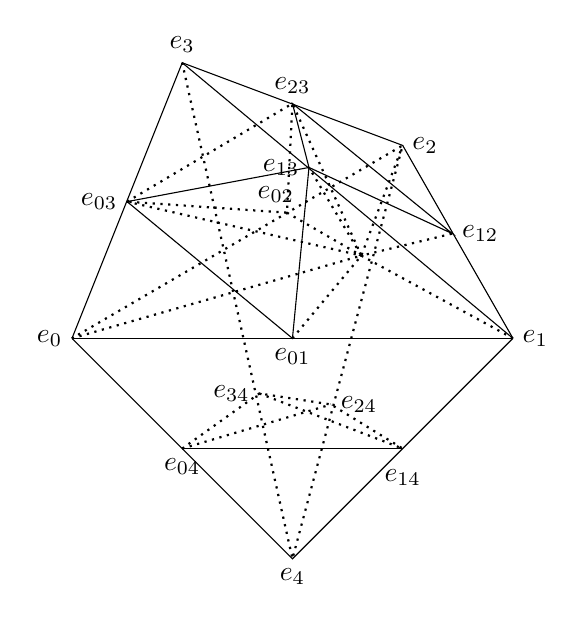
\begin{tikzpicture}[scale=0.7]
    \draw[] (0,0)--(8,0);
   \draw[] (0,0)--(4,-4)--(8,0);  
 \draw[] (0,0)--(2,5)--(8,0);
 \draw[] (2,5)--(6,3.5)--(8,0);
 \draw[thick, dotted] (2, 5)--(4, -4)--(6, 3.5)--(0,0);
  \draw[] (1,2.48)--(4,0)--(4.3,3.1)--(1,2.48);
    \draw[thick, dotted] (1,2.48)--(5.25, 1.5)--(4, 4.26);
   \draw[thick, dotted] (1,2.48)--(4, 4.26)--(3.9, 2.28)--(1,2.48);
    \draw[thick, dotted] (3.9, 2.28)--(5.25, 1.5);
     \draw[thick, dotted] (0, 0)--(5.25, 1.5)--(4.3,3.1);
   \draw[thick, dotted] (8, 0)--(5.25, 1.5)--(6.9, 1.9);
   \draw[thick, dotted] (4, 0)--(5.25, 1.5)--(6, 3.5);
   
    \node[left] at (0,0) {$e_0$};
   \node[below] at (4, -4) {$e_4$};
       \node[right] at (8,0) {$e_1$};
   \node[right] at (6, 3.5) {$e_2$};
    \node[above] at (2,5) {$e_3$};
  \node[right] at (6.9, 1.9) {$e_{12}$};
     \node[above] at (4, 4.26) {$e_{23}$};
       \node[below] at (6,-2.2) {$e_{14}$};
   \node[left] at (3.4,-1) {$e_{34}$};
     \node[left] at (4.3,3.1) {$e_{13}$}; 
 \node[right] at (4.7,-1.2) {$e_{24}$};
     \node[left] at (1,2.48) {$e_{03}$};
    \node[below] at (4,0) {$e_{01}$};
  \node[above] at (3.7, 2.28) {$e_{02}$};
   \node[below] at (2,-2) {$e_{04}$};
   \draw[] (2,-2)--(6,-2); 
    \draw[thick, dotted] (2,-2)--(3.4,-1)--(4.7,-1.2)--(6,-2); 
     \draw[] (4.3, 3.1)--(4.3,3.1)--(6.9, 1.9)--(4, 4.26)--(4.3, 3.1); 
        \draw[thick, dotted] (2,-2)--(4.7,-1.2); 
   \draw[thick, dotted] (3.4,-1)--(6,-2); 
 \end{tikzpicture}
\caption{A part of a triangulation on $\Delta^4$.}
\label{fig_trin_D4}
 \end{figure}
 Let $e_{ij}$ (resp., $e_{ijk}$) denote the barycenter of the simplex  $e_ie_j$ (resp., $e_ie_je_k$) in $\D^4$ for $i,j,k\in \{0,\ldots,4\}$. 
The induced triangulation on $F_0=\mathrm{Ind}_{\D^4}(\{e_1,e_2,e_3,e_4\}) $ contains the faces as in Figure \ref{fig_Tring_F0}. 
 \begin{figure}
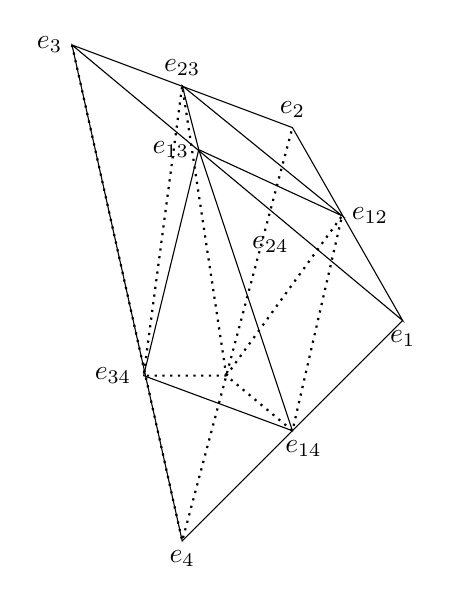
\begin{tikzpicture}[scale=0.7]
 \draw[] (2,5)--(6,3.5)--(8,0)--(2,5)--(4,-4)--(8,0);
 \draw[thick, dotted] (2, 5)--(4, -4)--(6, 3.5);
 \draw[] (4.3, 3.1)--(6,-2)--(3.3,-1)--(4.3,3.1)--(6.9, 1.9)--(4, 4.26)--(4.3, 3.1);
 \draw[thick, dotted] (4.8, -1)--(6.9, 1.9)--(6,-2)--(4.8, -1)--(3.3,-1)--(4, 4.26)--(4.8, -1);

 \node[right] at (6.9, 1.9) {$e_{12}$};
   \node[above] at (6, 3.5) {$e_2$};
    \node[above] at (4, 4.26) {$e_{23}$};
  \node[below] at (4,-4) {$e_4$};
    \node[below] at (8,0) {$e_1$};
      \node[below] at (6.2,-2) {$e_{14}$};
   \node[left] at (2,5) {$e_{3}$};
   \node[left] at (3.25,-1) {$e_{34}$};
     \node[left] at (4.3,3.1) {$e_{13}$}; 
 \node[below] at (5.6, 1.7) {$e_{24}$};
    
\end{tikzpicture}
\caption{A triangulation on $F_0$.}
\label{fig_Tring_F0}
 \end{figure}
Suppose that there is an edge between $e_{12}$ and $e_{34}$, say $e_{12}e_{34}$. Then $(-1, -1, 0,0)(e_{12}e_{34})=(-e_{12})e_{34}$ is also an edge in $X$. This is a contradiction, since $e_{12}=-e_{12}$ in $\mathbb{RP}^4$. By similar arguments, there cannot be an edge between $e_{14}$ and $e_{23}$. 

Now, to obtain the induced triangulation of $\Delta^4$, we need to have edges either from $e_{012}$ to each of $e_{03}, e_{23}, e_{24}$, or from $e_{134}$ to each of vertices $e_{02}, e_{13}, e_{23}$. However, similarly as above, there cannot be an edge between the vertices  $e_{23}$, $e_{012}$, $e_{34}$, $e_{034}$, and $e_{23}$. Observe that the tetrahedron $e_{13}e_{14}e_{012}e_{034}$ is a simplex in $X$. So, it is a face of two $4$-simplices. The other vertex of these two simplices should come from $\{e_{24}, e_{34}, e_{12}, e_{23}\}$. Now, $e_{13}e_{14}e_{012}e_{034}e_{24}$ cannot be a $4$-simplex, since $e_{13}e_{24}$ is not an edge in $X$. Similarly, $e_{13}e_{14}e_{012}e_{034}e_{34}$, $e_{13}e_{14}e_{012}e_{034}e_{12}$, and $e_{13}e_{14}e_{012}e_{034}e_{23}$ cannot be a $4$-simplex  $\Delta^4$. Therefore, there is no $16$-vertex $\ZZ_2^4$-equivariant triangulation of $\mathbb{R}P^4$.

If $Y$ is a $17$-vertex equivariant triangulation of $\mathbb{R}P^4$, then one vertex of $Y$ has to be a fixed vertex (see Lemma \ref{lem1}), say $e_0$. The situation of the vertices in $V(Y)\setminus\{e_0\}$ will be as in the case for $X$ above. Thus, by similar arguments,  $Y$ cannot exist.  
\end{proof}

\end{document}
